%%%%%%%%%%%%%%%%%%%%%%%%%%%%%%%%%%%%%%%%%
% Short Sectioned Assignment
% LaTeX Template
% Version 1.0 (5/5/12)
%
% This template has been downloaded from:
% http://www.LaTeXTemplates.com
%
% Original author:
% Frits Wenneker (http://www.howtotex.com)
%
% License:
% CC BY-NC-SA 3.0 (http://creativecommons.org/licenses/by-nc-sa/3.0/)
%
%%%%%%%%%%%%%%%%%%%%%%%%%%%%%%%%%%%%%%%%%

%----------------------------------------------------------------------------------------
%	PACKAGES AND OTHER DOCUMENT CONFIGURATIONS
%----------------------------------------------------------------------------------------

\documentclass[paper=a4, fontsize=11pt]{scrartcl} % A4 paper and 11pt font size

\usepackage[T1]{fontenc} % Use 8-bit encoding that has 256 glyphs
%\usepackage{fourier} % Use the Adobe Utopia font for the document - comment this line to return to the LaTeX default
\usepackage[english]{babel} % English language/hyphenation
\usepackage{amsmath,amsfonts,amsthm} % Math packages
\usepackage{mathtools} %More math! (For dscases)
\usepackage{hyperref} %HTML package
\usepackage{pgfplots} %Makes plots in LaTeX
\usepackage{tikz} %Also tikz?
\usepgfplotslibrary{fillbetween}%Let's me fill between named plots
\usepackage{graphicx} %import pics
\graphicspath{ {Python_figs/} }
\DeclareGraphicsExtensions{.pdf,.png,.jpg}
\usepackage{sectsty} % Allows customizing section commands
\allsectionsfont{ \normalfont\scshape} % Make all sections the default font and small caps


\renewcommand{\thesubsection}{\alph{subsection}} %Make subsections start with letters

\usepackage{fancyhdr} % Custom headers and footers
\pagestyle{fancyplain} % Makes all pages in the document conform to the custom headers and footers
\fancyhead{} % No page header - if you want one, create it in the same way as the footers below
\fancyfoot[L]{} % Empty left footer
\fancyfoot[C]{} % Empty center footer
\fancyfoot[R]{\thepage} % Page numbering for right footer
\renewcommand{\headrulewidth}{0pt} % Remove header underlines
\renewcommand{\footrulewidth}{0pt} % Remove footer underlines
\setlength{\headheight}{13.6pt} % Customize the height of the header

\numberwithin{equation}{section} % Number equations within sections (i.e. 1.1, 1.2, 2.1, 2.2 instead of 1, 2, 3, 4)
\numberwithin{figure}{section} % Number figures within sections (i.e. 1.1, 1.2, 2.1, 2.2 instead of 1, 2, 3, 4)
\numberwithin{table}{section} % Number tables within sections (i.e. 1.1, 1.2, 2.1, 2.2 instead of 1, 2, 3, 4)

\setlength\parindent{0pt} % Removes all indentation from paragraphs - comment this line for an assignment with lots of text

%----------------------------------------------------------------------------------------
%	TITLE SECTION
%----------------------------------------------------------------------------------------

\newcommand{\horrule}[1]{\rule{\linewidth}{#1}} % Create horizontal rule command with 1 argument of height

\title{	Assignment 4}

\author{Benjamin Jakubowski} % Your name

\date{\normalsize\today} % Today's date or a custom date

\begin{document}

\maketitle % Print the title

%----------------------------------------------------------------------------------------
%	PROBLEM 1
%----------------------------------------------------------------------------------------

\section{Basketball}

\subsection{Probability Curry makes his $14^{th}$ shot}

Let $X_i$ represent Curry's $i^{th}$ shot. Then
\[
X_i = 
\begin{dcases}
   1 & \textrm{  if he makes it}\\
   0 & \textrm{  if he misses}\\
\end{dcases}
\]
Now,
\[
P_{X_{i+1}}(1) = 
\begin{dcases}
   .6 & \textrm{  if } X_i = 1\\
   .3 & \textrm{  if } X_i = 0\\
\end{dcases}
\]
Thus, the only shot that matters when predicting the $i+1^{st}$ shot is the outcome of the $i^{th}$ shot. Therefore, when predicting the outcome of the $14^{th}$ shot given the outcomes of the $2^{nd}$ and $12^{th}$, the outcome of the $12^{th}$ shot provides all necessary information- knowing the outcome of the second shot gives no additional information.  (More formally, let $m, n \in \{1,2,... j-1\}$ and $m > n$. Then $P(X_j | X_{m}, X_{n}) = P(X_j | X_{m})$.)

Now, since $X_{12} = 1$,
\[
P_{X_{13} | X_{12} = 1} (x) =
\begin{dcases}
   .6 & \textrm{  for } x = 1\\
   .4 & \textrm{  for } x = 0 
\end{dcases}
\]
Moreover,
\begin{align*}
P_{X_{14} | X_{13} = 1} (1) &= .6\\
P_{X_{14} | X_{13} = 0} (1) &= .3
\end{align*}

Therefore,
\begin{align*}
P_{X_{14}} (1) &= P_{X_{14} | X_{13} = 0} (1) \cdot  P_{X_{13} | X_{12} = 1} (0) + P_{X_{14} | X_{13} = 1} (1) \cdot  P_{X_{13} | X_{12} = 1} (1)\\
   &= .3 \cdot .4 + .6 \cdot .6 = .12 + .36 = .48
\end{align*}

\subsection{Probability Curry made his $1^{st}$ shot}

First, note $P(X_1 = 1 | X_3 = 0, X_9 = 0) = P(X_1 = 1 | X_3 = 0)$. Then $P(X_1 = 1 | X_3 = 0)$

\begin{align*}
   &\qquad {}= \frac{P(X_3 = 0 | X_1 = 1) P(X_1 = 1)}{P(X_3 = 0)} \\
   &\qquad {}= \frac{\left(P(X_3 = 0 | X_2 = 0) P(X_2 = 0 | X_1 = 1) + P(X_3 = 0 | X_2 = 1) P(X_2 = 1 | X_1 = 1) \right) P(X_1 = 1)}{P(X_3 = 0)}
\end{align*}

And
\begin{align*}
P(X_3 = 0) &= P(X_3 = 0 | X_2 = 0) P(X_2 = 0 | X_1 = 0)P(X_1 = 0) 
   \\& \qquad {} + P(X_3 = 0 | X_2 = 1) P(X_2 = 1 | X_1 = 0)P(X_1 = 0) 
   \\& \qquad {} + P(X_3 = 0 | X_2 = 0) P(X_2 = 0 | X_1 = 1)P(X_1 = 1)
   \\& \qquad {} + P(X_3 = 0 | X_2 = 1) P(X_2 = 1 | X_0 = 1)P(X_1 = 1) \\
   &= .7 \cdot .7 \cdot .6 + .4 \cdot .3 \cdot .6 + .7 \cdot .4 \cdot .4 + .4 \cdot .6 \cdot .4\\
   &= .294 + .072 + .112 + .096\\
   &= .574
\end{align*}

Thus, $P(X_1 = 1 | X_3 = 0)$
\begin{align*}
&\qquad {}=  \frac{\left(P(X_3 = 0 | X_2 = 0) P(X_2 = 0 | X_1 = 1) + P(X_3 = 0 | X_2 = 1) P(X_2 = 1 | X_1 = 1) \right) P(X_1 = 1)}{P(X_3 = 0)} \\
   &\qquad {}=  \frac{\left(.7 \cdot .4 + .4 \cdot .6 \right) \cdot .4 }{.574} \\
   &\qquad {}=  \frac{.52 \cdot .4 }{.574} = .36237
\end{align*}

\subsection{Expected number of consecutive baskets}

Let $Y$ be the number of shots made in a row following the first shot. Then
\begin{align*}
E(Y) &= E(E(Y | X_1))\\
   &= E(Y | X_1 = 0) \cdot P(X_1 = 0) + E(Y | X_1 = 1) \cdot P(X_1 = 1)\\
   &= E(Y | X_1 = 0) \cdot .6 + E(Y | X_1 = 1) \cdot .4
\end{align*}

Next, note
\begin{equation*}
E(Y | X_1 = 0) = \sum_{y = 0}^\infty y \cdot P(Y = y | X_1 = 0)
\end{equation*}
and
\[
P_{Y | X_1 = 0}(y) = 
\begin{dcases}
   .7 & \textrm{  for } y =0\\
   .3 \cdot .6^{y-1} \cdot .4 & \textrm{  for } y \geq 1\\
\end{dcases}
\]
Therefore, 
\begin{align*}
E(Y | X_1 = 0) &= \sum_{y = 0}^\infty y \cdot P(Y = y | X_1 = 0)\\
   &= 0 \cdot .7 + \sum_{y = 1}^\infty (y \cdot .3 \cdot .6^{y-1} \cdot .4)\\
   &= .3 \cdot .4 \cdot \sum_{y = 1}^\infty (y \cdot .6^{y-1})\\
   &= .3 \cdot .4 \cdot \frac{1}{.6} \cdot \sum_{y = 1}^\infty (y \cdot .6^{y})\\
   &= .3 \cdot .4 \cdot \frac{1}{.6} \cdot \frac{.6}{(1-.6)^{.2}}\\
   &= .75
\end{align*}

Similarly, note
\begin{equation*}
E(Y | X_1 = 1) = \sum_{y = 0}^\infty y \cdot P(Y = y | X_1 = 1)
\end{equation*}
and
\[
P_{Y | X_1 = 1}(y) = .6^y \cdot .4 \textrm{  for } y \geq 0
\]
Therefore
\begin{align*}
E(Y | X_1 = 1) &= \sum_{y = 0}^\infty y \cdot P(Y = y | X_1 = 1)\\
   &=  \sum_{y = 0}^\infty (y \cdot .6^{y} \cdot .4)\\
   &= .4 \cdot \sum_{y = 0}^\infty (y \cdot .6^{y})\\
   &= .4 \cdot \frac{.6}{(1-.6)^{.2}}\\
   &= 1.5
\end{align*}

Finally,
\[
E(Y) = E(Y | X_1 = 0) \cdot .6 + E(Y | X_1 = 1) \cdot .4 = .75 \cdot .6 + 1.5 \cdot .4 = 1.05
\]

Therefore, we expect Curry to make 1.05 shots in a row regardless of whether he makes the first shot or not.

%----------------------------------------------------------------------------------------
%	PROBLEM 2
%----------------------------------------------------------------------------------------

\section{Model}

\subsection{Finding $P_N$ and $P_C$}

First, we find $P_N$:
\begin{align*}
P_N(n) &= \sum_{k = 0}^n \sum_{c \in \{1/4, 4/5\}} P_{N, C, K}(n,c,k)\\
   &= \sum_{k = 0}^n \left[\frac{1}{30}{n \choose k}(1/4)^{k}(3/4)^{n-k} + \frac{1}{60}{n \choose k}(4/5)^{k}(1/5)^{n-k} \right] \\
   &= \frac{1}{30}\sum_{k = 0}^n \left[{n \choose k}(1/4)^{k}(3/4)^{n-k} \right] + \frac{1}{60} \sum_{k = 0}^n \left[{n \choose k}(4/5)^{k}(1/5)^{n-k} \right] \\
   &= \frac{1}{30} \cdot 1 + \frac{1}{60} \cdot 1= 1/20
\end{align*}

Next, we find $P_C$:
\begin{align*}
P_C(c) &=
\begin{dcases}
& \sum_{n = 1}^{20} \left[ \sum_{k = 0}^{n} \left(\frac{1}{30}{n \choose k}(1/4)^{k}(3/4)^{n-k} \right) \right] \textrm{  for } c = 1/4 \\
& \sum_{n = 1}^{20} \left[ \sum_{k = 0}^{n} \left(\frac{1}{60}{n \choose k}(4/5)^{k}(1/5)^{n-k} \right) \right] \textrm{  for } c = 4/5 \\
\end{dcases}\\
&=
\begin{dcases}
& \sum_{n = 1}^{20} \frac{1}{30} =  \frac{20}{30} = \frac{2}{3}  \textrm{  for } c = 1/4 \\
& \sum_{n = 1}^{20}  \frac{1}{60} =\frac{20}{60} = \frac{1}{3}  \textrm{  for } c = 4/5 \\
\end{dcases}
\end{align*}

Finally, we will show $P_{N,C}(n,c) = P_N(n) \cdot P_C(c)$ (and, as such, $C$ and $N$ are independent):
\begin{align*}
P_{N,C}(n,c) &= \sum_{k = 0}^n P_{N, C, K} (n, c, k) \\
   &=
   \begin{dcases}
   & \sum_{k = 0}^{n} \frac{1}{30}{n \choose k}(1/4)^{k}(3/4)^{n-k} \textrm{  for } c = 1/4 \\
   & \sum_{k = 0}^{n} \frac{1}{60}{n \choose k}(4/5)^{k}(1/5)^{n-k} \textrm{  for } c = 4/5 \\
   \end{dcases}\\
   &=
   \begin{dcases}
   & \frac{1}{30} \textrm{  for } c = 1/4 \\
   & \frac{1}{60} \textrm{  for } c = 4/5
   \end{dcases}
\end{align*}

But then note:
\[
P_{N,C}(n,c) = 
 \begin{dcases}
   & \frac{1}{30} = \frac{1}{20} \cdot \frac{2}{3} = P_N(n) \cdot P_C(c) \textrm{  for } c = 1/4, n \in \{1, 2, ... 20\} \\
   & \frac{1}{60} = \frac{1}{20} \cdot \frac{1}{3} = P_N(n) \cdot P_C(c) \textrm{  for } c = 4/5, n \in \{1, 2, ... 20\} 
   \end{dcases}
\]
Thus, $C$ and $N$ are independent

\subsection{Real-life example}

This model could correspond to the following scenario:
\begin{enumerate}
   \item C: Pick one of two biased coins. Specifically, pick:
      \begin{itemize}
         \item Coin 1 with probability 2/3. This coin flips heads with probability 1/4.
         \item Coin 2 with probability 1/3. This coin flips heads with probability 4/5.
      \end{itemize}
   \item N: Spin a fair (i.e. random uniform) spinner, numbered 1 to 20, to determine how many times to flip said coin. 
   \item K: Count the number of heads in your N flips.
\end{enumerate}

This scenario would be well modeled by the joint pmf given in the problem.

\subsection{Condition PMF $P_{N | K, C}$}

First, note
\[P(N = n | C = c, K = k) = \frac{P(N = n, C = c, K = k)}{P(C = c, K = k)}\]

Thus, to proceed we first determine:
\begin{align*}
P_{C, K}(c,k) &= \sum_{n = 0}^{20} P_{N, C, K}(n, c, k)\\
   &=
   \begin{dcases}
      & \sum_{n = 1}^{20} 1/30 {n \choose k} (1/4)^k (3/4)^{n-k} \textrm{  for } c = 1/4\\
      & \sum_{n = 1}^{20} 1/60 {n \choose k} (4/5)^k (1/5)^{n-k} \textrm{  for } c = 4/5
   \end{dcases}
\end{align*}
Therefore:
\begin{align*}
P_{N | C, K}(n | c,k) &=
   \begin{dcases}
      & \frac{1/30 {n \choose k}(1/4)^k (3/4)^{n-k}}{1/30 (1/4)^k \sum_{n = 1}^{20} {n \choose k} (3/4)^{n-k}} \textrm{  for } c = 1/4 \\
      & \frac{1/60 {n \choose k}(4/5)^k (1/5)^{n-k}}{1/60 (4/5)^k \sum_{n = 1}^{20} {n \choose k} (1/5)^{n-k}} \textrm{  for } c = 4/5
   \end{dcases}
   \\
    &= 
     \begin{dcases}
      & \frac{{n \choose k}(3/4)^{n-k}}{\sum_{n = 1}^{20} {n \choose k} (3/4)^{n-k}} \textrm{  for } c = 1/4 \\
      & \frac{{n \choose k}(1/5)^{n-k}}{\sum_{n = 1}^{20} {n \choose k} (1/5)^{n-k}} \textrm{  for } c = 4/5
   \end{dcases}
\end{align*}


\subsection{Plotting the distribution $P_{N | K, C}$}
 
Below are plots of the distribution of $N$ given $K = 1, K = 10, K = 19$ and $C = 1/4$ on one graph and $K = 1, K = 10, K = 19$ and $C = 4/5$ on another graph.
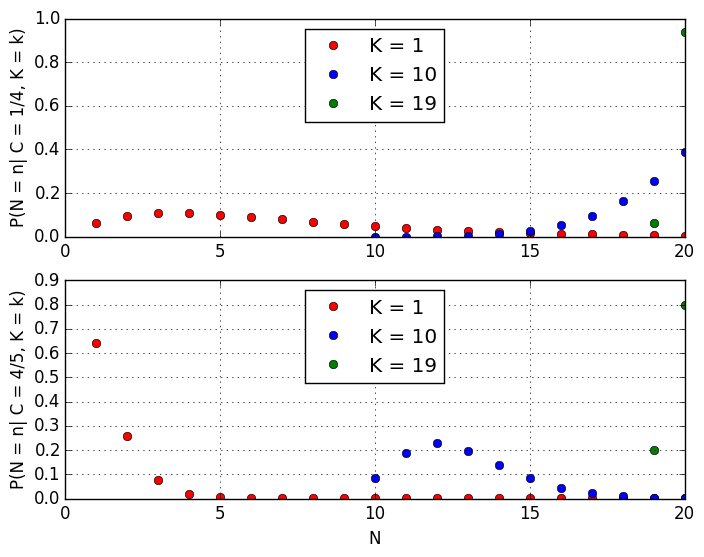
\includegraphics[scale=0.83]{Q2d_fig}
These results make intuitive sense in the context of the example posed in question b. First, comparing the PMFs when $C = 4/5$ and $C = 1/4$, it is clear that for any $K = k$ lower values of $N$ are more likely when $C = 4/5$ than when $C = 1/4$. More specifically, it is apparent from the plots that given any $K = k$, for any value $x$ such that  $k \leq x < 20$
\[P(N \leq x | C = 1/4) < P(N \leq x | C = 4/5)\]
In the context of the problem, that makes sense- if you get heads with probability 4/5, you'd expect to need fewer flips to get $k$ heads than you would if you had the coin with 1/4 probability of heads.

%----------------------------------------------------------------------------------------
%	PROBLEM 3
%----------------------------------------------------------------------------------------

\section{Router}

\subsection{Mean and variance of number of packets}

Let  $N$ be the number of packets that arrive at the router in a second. Note $N \sim \textrm{Pois}(\lambda)$.
Let $X$ be the number of packets routed through connection 1. Then $X \sim \textrm{B}(N,p)$.
 
Now we can find the mean and variance of $X$:
\begin{align*}
E(X) &= E(E(X | N))\\
   &= E(N \cdot p) = p \cdot E(N) = p \cdot \lambda \\
Var(X) &= E(Var(X | N)) + Var(E(X | N))\\
   &= E(N \cdot p \cdot (1-p)) + Var(N \cdot p)\\
   &= p \cdot (1-p) \cdot E(N) + p^2 \cdot Var(N)\\
   &= p \cdot (1-p) \cdot  \lambda + p^2 \cdot \lambda\\
   &= p \cdot \lambda
\end{align*}
Thus, $E(X) = Var(X) = p \cdot  \lambda$. 

\subsection{PMF of number of packets}

The PMF $P_X(x)$ is
\begin{equation*}
P_X(x) = \sum_{n=0}^\infty P(X = x | N = n) \cdot P(N = n)
\end{equation*}
Note since $N \geq X$ by definition, this is equivalent to
\begin{align*}
P_X(x) &= \sum_{n=x}^\infty \left[{n \choose x} p^x (1-p)^{n-x} \cdot \frac{\lambda^n}{n!} e^{-\lambda}\right] \\ 
   &= p^x e^{-\lambda} \cdot \sum_{n=x}^\infty \left[ \frac{n!}{(n-x)!x!} \cdot (1-p)^{n-x} \cdot \frac{\lambda^n}{n!} \right] \\ 
   &= \frac{p^x e^{-\lambda}}{x!} \cdot \sum_{n=x}^\infty \left[ \frac{(1-p)^{n-x}}{(n-x)!} \cdot \lambda^n \right] \\ 
   &= \frac{p^x e^{-\lambda}}{x!} \cdot \sum_{n=x}^\infty \left[ \frac{(1-p)^{n-x}}{(n-x)!} \cdot \lambda^{n-x} \cdot \lambda^x \right] \\ 
   &= \frac{p^x e^{-\lambda} \lambda^x}{x!} \cdot \sum_{n=x}^\infty \left[ \frac{\left[(1-p) \lambda \right]^{n-x}}{(n-x)!} \right] \\ 
   &= \frac{p^x e^{-\lambda} \lambda^x}{x!} \cdot \sum_{n=0}^\infty \left[ \frac{\left[(1-p) \lambda \right]^{n}}{n!} \right] \\
   &= \frac{p^x e^{-\lambda} \lambda^x}{x!} e^{(1-p) \cdot \lambda}\\
   &= \frac{(p \lambda) ^x}{x!} e^{\lambda - p \lambda - \lambda} = \frac{(p \lambda) ^x}{x!} e^{- p \lambda}
\end{align*}

Thus, $P_X(x) = \frac{(p \lambda) ^x}{x!} e^{- p \lambda}$ and $X \sim \textrm{Pois}(p \lambda)$.

%----------------------------------------------------------------------------------------
%	PROBLEM 4
%----------------------------------------------------------------------------------------

\section{Cheap GPS}

\subsection{Finding precision $\Delta_1$}

First, recall Jennifer has defined the precision of the location estimate as the smallest $\Delta$ such that the probability of the error being larger than $\Delta$ is smaller than 1\%.

Thus, using $X_i$ as an estimator of $d_i$, we want to find $\Delta$ such that:
\begin{align*}
P(|X_i - d_i| > \Delta) &< .01 \\
P(|Z_i| > \Delta) &< .01
\end{align*}
Using Chebyshev's inequality, we know
\[ P(|Z_i - E(Z_i)| > a) \leq \frac{Var(Z_i)}{a^2}\]
Thus 
\[P(|Z_i - E(Z_i)| = |Z_i - 0| = |Z_i| > \Delta) < \frac{1}{\Delta^2}\]
So $P(|Z_i| > \Delta) < 0.1$ when $\Delta \geq 10$. Hence, the precision $\Delta_1$ of using $X_i$ as an estimate of $d_i$ is $\Delta_1 = 10$.

\subsection{Finding precision $\Delta_2$}

First,
\begin{align*}
Y_i &= \frac{1}{m} \sum_{j = i - (m-1)}^{i} X_i \\
   &=  \frac{1}{m} \sum_{j = i - (m-1)}^{i} \left(d_j + Z_j \right) \\
   &=  \frac{1}{m} \sum_{j = i - (m-1)}^{i} \left(d_j \right) +\frac{1}{m} \sum_{j = i - (m-1)}^{i} \left(Z_j \right)
\end{align*}

Let's consider just
\[\sum_{j = i - (m-1)}^{i} \left(d_j \right) \]

First, since Mary never moves backward and has a maximum speed of 2 meters per second,
\[d_{i} - 2(n) \leq d_{i-n} \leq d_{i} \]

Thus, we can place the following bound on the sum of the $d_j$s:
\begin{alignat*}{3}
\sum_{j = i - (m-1)}^{i} \left(d_i - 2 (i-j) \right) && \leq \sum_{j = i - (m-1)}^{i} d_j \textrm{ }&& \leq \sum_{j = i - (m-1)}^{i} d_i \\
m \cdot d_i - 2\sum_{j = i - (m-1)}^{i} \left(i-j \right) && \leq \sum_{j = i - (m-1)}^{i} d_j \textrm{ }&& \leq \sum_{j = i - (m-1)}^{i} d_i \\
m \cdot d_i - 2\sum_{j = 0}^{m-1} \left(j \right) && \leq \sum_{j = i - (m-1)}^{i} d_j \textrm{ }&& \leq \sum_{j = i - (m-1)}^{i} d_i \\
m \cdot d_i - 2 \frac{(m-1)m}{2} && \leq \sum_{j = i - (m-1)}^{i} d_j \textrm{ }&& \leq \sum_{j = i - (m-1)}^{i} d_i \\
m \cdot d_i - (m-1)m && \leq \sum_{j = i - (m-1)}^{i} d_j \textrm{ }&& \leq \sum_{j = i - (m-1)}^{i} d_i
\end{alignat*}

Now recall
\[Y_i = \frac{1}{m} \sum_{j = i - (m-1)}^{i} d_j + \frac{1}{m} \sum_{j = i - (m-1)}^{i} Z_j\]
Therefore, multiplying by $\frac{1}{m}$ and adding $\frac{1}{m} \sum_{j = i - (m - 1)}^{i} Z_j$ throughout bounds $Y_i$:
\[
\frac{1}{m} \left( m \cdot d_i - (m-1)m \right) +\frac{1}{m} \sum_{j = i - (m - 1)}^{i} Z_j \leq \textrm{ } Y_i   \textrm{ } \leq \frac{1}{m} \sum_{j = i - (m-1)}^{i} d_i + \frac{1}{m}  \sum_{j = i - (m - 1)}^{i} Z_j\]
Simplifying, we get
\[
d_i - (m-1) +\frac{1}{m}  \sum_{j = i - (m - 1)}^{i} Z_j \leq \textrm{ }  Y_i  \textrm{ }  \leq \frac{1}{m} \cdot m \cdot d_i +  \frac{1}{m} \sum_{j = i - (m - 1)}^{i} Z_j\]
\[
-(m-1) +\frac{1}{m}  \sum_{j = i - (m - 1)}^{i} Z_j \leq \textrm{ }  Y_i - d_i \textrm{ }  \leq  \frac{1}{m} \sum_{j = i - (m - 1)}^{i} Z_j\]

This implies

\[ \left|Y_i - d_i \right| \leq \textrm{max}\left\{\left| -(m-1) + \frac{1}{m} \sum_{j = i - (m-1)}^{i} Z_j \right|, \left| \frac{1}{m} \sum_{j = i - (m-1)}^{i} Z_j \right| \right\}\]

But, by the triangle inequality,
\[ \left| -(m-1) + \frac{1}{m} \sum_{j = i - (m-1)}^{i} Z_j \right| \leq \left| m-1 \right| + \left| \frac{1}{m} \sum_{j = i - (m-1)}^{i} Z_j \right| \]

Thus, we have
\[ \left|Y_i - d_i \right| \leq \left| m-1 \right| + \left| \frac{1}{m} \sum_{j = i - (m-1)}^{i} Z_j \right| \]

That implies (noting $m \geq 1$)

\[ P( \left|Y_i - d_i \right| > \Delta ) \leq P\left( \left| m-1 \right| + \left| \frac{1}{m} \sum_{j = i - (m-1)}^{i} Z_j \right| > \Delta \right) = P\left( \left| \frac{1}{m} \sum_{j = i - (m-1)}^{i} Z_j \right| > \Delta - (m - 1)\right) \]

Now let's let
\[X = \frac{1}{m} \sum_{j = i - (m-1)}^{i} Z_j \]

Then $E(X) = 0$ (since $E(Z_j) = 0$ and expectation is a linear operator), and (by the independence of the $Z_j$s)
\[Var(X) =  \sum_{j = i - (m-1)}^{i} Var\left( \frac{1}{m} Z_j\right) = \sum_{j = i - (m-1)}^{i} \frac{1}{m^2} Var(Z_j) = 0\]

Now, setting
\[P\left( \left|X\right| > \Delta - (m-1) \right) \leq 0.01\]
Chebyshev's inequality implies
\[0.01 \geq \frac{Var(X)}{(\Delta - (m-1))^2}\]

Thus

\[(\Delta_2 - (m-1))^2 = \frac{100}{m} \implies \Delta_2 = 10 \cdot m^{-1/2} + m - 1 \]

\subsection{Evaluating $\Delta_2$ for $m = 4$}

When $m = 4$,
\[\Delta_2 = 10 \cdot m^{-1/2} + m - 1 = 10 \cdot (4)^{-1/2} + 4 - 1 = 8 \]

That's why Jennifer is using the running mean- it's an improved estimator of $d_i$ (in the sense it is more precise, though it is unfortunately biased assuming Mary's speed is non-zero).

\subsection{Minimizing $\Delta_2$ fusing the running mean}
First, let's express $\Delta_2$ as a function of $m$:
\[\Delta_2(m) = 10 \cdot m^{-1/2} + m - 1\]
Then
\begin{align*}
\Delta_2(1) &= 10\\
\Delta_2(2) &\approx 8.071\\
\Delta_2(3) &\approx 7.7735\\
\Delta_2(4) &= 8
\end{align*}
Finally, note $\textrm{d}\Delta_2/\textrm{d}m = -5 m^{-3/2} + 1 > 0$ for all $n \in \mathbb{N}, n \geq 4$. Thus, $\Delta_2$ is strictly increasing from $4$ to $\infty$. Hence, the best precision Jennifer can achieve using a running mean is $\Delta_2(3) \approx 7.7735$.

%----------------------------------------------------------------------------------------
%	PROBLEM 5
%----------------------------------------------------------------------------------------

\section{Iterated Expectation for Random Vectors}

\subsection{Proof for disjoint random vectors}

We will show that for any disjoint subvectors indexed by ${\mathcal{I}}, {\mathcal{J}} \subseteq \{1, 2, ..., n\}, {\mathcal{I}} \cap {\mathcal{J}} = \emptyset$,

\[E(E(\mathbf{X_{\mathcal{I}}} | \mathbf{X_{\mathcal{J}}})) = E(\mathbf{X_{\mathcal{I}}})\]

Note we will demonstrate this in the continuous case- the discrete case is similar (replacing integrals with sums). 

First, let
\begin{align*}
h(\vec{x_{\mathcal{J}}}) &:= E(\mathbf{X_{\mathcal{I}}} | \mathbf{X_{\mathcal{J}}} = \vec{x_{\mathcal{J}}})\\
   &= \int_{\mathbf{{\mathcal{I}}}} \vec{x_{\mathcal{J}}} \cdot f_{ \mathbf{X_{\mathcal{I}} | X_{\mathcal{J}}}}(\vec{x_{\mathcal{I}}} | \vec{x_{\mathcal{J}}}) \mathbf{d}\vec{x_{\mathcal{I}}}
\end{align*}

Before we proceed, let's clarify this abuse of notation:
\[ \int_{\mathbf{{\mathcal{I}}}} \textrm{ represents  } \int_{x_{{\mathcal{I}}_{1}} = -\infty}^\infty \int_{x_{{\mathcal{I}}_{2}} = -\infty}^\infty ... \int_{x_{{\mathcal{I}}_{i}} = -\infty}^\infty \]
\[ \mathbf{d}\vec{x_{\mathcal{I}}} \textrm{ represents  } \textrm{d} x_{{\mathcal{I}}_{i}}  \textrm{d} x_{{\mathcal{I}}_{i-1}} ...  \textrm{ d} x_{{\mathcal{I}}_{1}}\]

Additionally, note that while $h(\vec{x_{\mathcal{J}}}) = E(\mathbf{X_{\mathcal{I}}} | \mathbf{X_{\mathcal{J}}} = \vec{x_{\mathcal{J}}})$ is a function mapping $\mathbb{R}^j \to \mathbb{R}^j$ (where $j$ is the length of $\vec{x_{\mathcal{J}}}$), $h(\mathbf{X_{\mathcal{J}}}) = E(\mathbf{X_{\mathcal{I}}} | \mathbf{X_{\mathcal{J}}})$ is a random vector (since a function of a random vector is itself a random vector).
Then
\begin{align*}
E(E(\mathbf{X_{\mathcal{I}}} | \mathbf{X_{\mathcal{J}}})) &= E(h(\mathbf{X_{\mathcal{J}}}))\\
   &= \int_{\mathbf{{\mathcal{J}}}} h(\vec{x_{\mathcal{J}}}) \cdot f_{ \mathbf{X_{\mathcal{J}}}}(\vec{x_{\mathcal{J}}})\mathbf{d}\vec{x_{\mathcal{J}}}\\
   &= \int_{\mathbf{{\mathcal{J}}}}\left( \int_{\mathbf{{\mathcal{I}}}} \vec{x_{\mathcal{I}}} f_{ \mathbf{X_{\mathcal{I}}} |  \mathbf{X_{\mathcal{J}}}}(\vec{x_{\mathcal{I}}} | \vec{x_{\mathcal{J}}}) \mathbf{d}\vec{x_{\mathcal{I}}} \right) \cdot f_{ \mathbf{X_{\mathcal{J}}}}(\vec{x_{\mathcal{J}}}) \mathbf{d}\vec{x_{\mathcal{J}}}\\
    &= \int_{\mathbf{{\mathcal{I}}}} \vec{x_{\mathcal{I}}} \left( \int_{\mathbf{{\mathcal{J}}}} f_{ \mathbf{X_{\mathcal{I}}} |  \mathbf{X_{\mathcal{J}}}}(\vec{x_{\mathcal{I}}} | \vec{x_{\mathcal{J}}}) \cdot f_{ \mathbf{X_{\mathcal{J}}}}(\vec{x_{\mathcal{J}}}) \mathbf{d}\vec{x_{\mathcal{J}}} \right) \mathbf{d}\vec{x_{\mathcal{I}}} \\
     &= \int_{\mathbf{{\mathcal{I}}}} \vec{x_{\mathcal{I}}} f_{ \mathbf{X_{\mathcal{I}}}}(\vec{x_t}) \mathbf{d}\vec{x_{\mathcal{I}}} \\
     &= E(\mathbf{X_{\mathcal{I}}})
\end{align*}

\subsection{Mean and Variance of K in Problem 2}

First, from question 2 we know
\begin{align*}
P_{K | N, C} &= \frac{P_{N, C, K}}{P_{N, C,}}\\
   &= {N \choose k} C^{k} (1 - C)^{N-k}
\end{align*}
So
\begin{align*}
E(K | N, C) &= \sum_{k = 0}^N k{N \choose k} C^{k} (1 - C)^{N-k}\\
   &= C\cdot N
\end{align*}

But then
\begin{align*}
E(K) &= E(E(K | N,C)) = E(CN)\\
   &= \sum_{n = 1}^{20} \sum_{c \in \{1/4, 4/5\}} c \cdot n \cdot P_{N, C} (n,c) \\
   &= \sum_{n = 1}^{20} \left[\frac{1}{4}\cdot n \cdot \frac{1}{30} + \frac{4}{5} \cdot n\cdot \frac{1}{60} \right] \\
   &= \sum_{n = 1}^{20} \frac{13}{600} \cdot n \\
   &= \frac{13 \cdot 20 \cdot 21}{600 \cdot 2} = 4.55
\end{align*}

Next, let's find the variance of $K$. First, note
\[Var(K) = E(K^2) - (E(K))^2\]
Well, $E(K^2) = E(E(K^2 | N, C))$, and
\[E(K^2 | N, C) = \sum_{k = 0}^N k^2 {N \choose k} C^k (1-C)^{N-k}\]

But this is just the second moment of a binomial (though, significantly, a binomial parameterized by random variables). Recall the variance of $B(N,C)$ is $NC(1-C)$. So
\begin{align*}
E(K^2 | N, C) &= Var(K | N, C) + (E(K | N, C))^2 \\
   &= NC(1-C) + (NC)^2
\end{align*}
Therefore,
\begin{align*}
E(K^2) &= E(E(K^2 | N, C)) \\
   &= \sum_{n = 1}^{20} \sum_{c \in \{1/4, 4/5\}} \left((n c (1-c) + (n c)^2) P_{N, C} (n,c)\right) \\
   &= \sum_{n = 1}^{20}\left[ \left(n \cdot \frac{1}{4} \cdot\frac{3}{4} + \left(n \cdot \frac{1}{4}\right)^2 \right) \frac{1}{30} + \left(n \cdot \frac{4}{5} \cdot \frac{1}{5} + \left(n \cdot \frac{4}{5}\right)^2 \right) \frac{1}{60} \right] \\
   &=  \sum_{n = 1}^{20}\left[ \left( \frac{3}{16} n + \frac{1}{16} n^2 \right) \frac{1}{30} + \left(\frac{4}{25}  n + \frac{16}{25} n^2 \right) \frac{1}{60} \right]\\
   &= 38.465
\end{align*}

So $Var(K) = E(K^2) - (E(K))^2 = 38.465 - (4.55)^2 = 17.7625$.
%----------------------------------------------------------------------------------------
\end{document}